\chapter[Equipe]{Equipe}

Para a criação do aplicativo montaremos uma equipe com 12 pessoas, profissionais da área de tecnologia, que trabalharão em pequenas partes do desenvolvimento. O conjunto das partes resultará no EducaLar.


\begin{figure}[htb]
	%\caption{\label{gantt}Placa Wiring S}
	\begin{center}
	    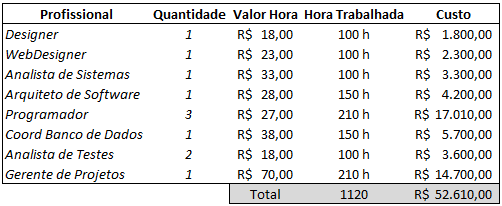
\includegraphics[scale=0.9]{tabelaCustos}
	\end{center}
	%\legend{Fonte: Site da 3GPP}
\end{figure}

%\begin{alineas}
%    \item Um Designer (ou \emph{Front End Designer}) %que é a pessoa %responsável por elaborar o desenho das interfaces do aplicativo.
%    \item Um Web designer %que vai ser responsável por aplicar o layout %projetado anteriormente.
%    \item Um Analista de sistemas %que vai ser responsável por %compreender a necessidade de negócio do cliente e especificar por %escrito o que precisa ser feito no projeto.
%    \item Um Arquiteto de software %que vai analisar as necessidades do %projeto e define a arquitetura técnica que melhor se encaixa no %projeto.
%    \item Cinco desenvolvedores/programadores %que vai transformar as %especificações de negócio do aplicativo em código sendo responsáveis %por 50 \% do esforço total do projeto de desenvolvimento e manutenção %do aplicativo.
%    \item Um analista de banco de dados %que vai tratar adequadamente %do grande volume de dados.
%    \item Um analista de testes %que vai fazer a validação do %aplicativo analisando todo sistema e vendo se não há erros %(\emph{bugs}) no aplicativo.
%    \item Gerente de projetos %que cria e acompanha o cronograma do %projeto, dando as diversas tarefas para os profissionais
%\end{alineas}